In this chapter, we will discuss reasoning, particularly the kind that involves
explicit discrete operations. The work we describe in
Chapters~\ref{chapter:wikitables} and~\ref{chapter:nlvr} employs discrete
operation based reasoning, and this chapter provides ncessary background.

\section{Learning to Reason with Latent Variables}
Reasoning involves making predictions related to the task at hand. Quite often,
the process goes through certain intermediate operations that lead to the final
prediction. Statistical reasoning models may model the intermediate operations as
estimating latent variables on which the final predictions are conditioned.
The latent variables may be continuous or discrete, and depending on the task at
hand, one choice may be more appropriate than the other. Using continuous latent
variables makes training easier since it is generally straight forward to use 
back-propagation. Discrete latent variable make training harder, as we discuss
later in this chapter, but it may be worth dealing with the difficulty in some
cases. Let us look at two examples to discuss the pros and cons of both the options.

First, consider an example from the Stanford Question Answering
Dataset (SQuAD)~\citep{Rajpurkar2016SQuAD10}, with the following context.
\begin{quote}
	\textit{Nikola Tesla (10 July 1856 – 7 January 1943) was a Serbian American
	inventor, electrical engineer, mechanical engineer, physicist, and
	futurist best known for his contributions to the design of the modern
	alternating current (AC) electricity supply system.}
\end{quote}
One question associated with this context is
\textit{In what year was Nikola Tesla born?}

Recent reading comprehension systems~\citep[among
others]{Seo2016BidirectionalAF,yu2018qanet} built for answering questions like
the one above, have sub-components that measure the relevance of various parts of
the queries to various parts of the corresponding contexts. This is typically
done using a soft attention mechanism~\citep{bahdanau:14}, that produces
(normalized) scores of query-context relevance. Relevance in these models is a 
\emph{continuous} latent variable, and thus its estimation is a continuous intermediate
operation. This setup lets the models learn diverse task specific patterns for
matching contexts and queries. For example, the model might assign a higher
relevance score to the span \textit{what year} in the question, and each of the
spans \textit{1856} and \textit{1943} in the context. This is a case where the
choice of continuous latent variables is more appropriate. 

On the other hand, consider the task of answering the following question given
the context below, an example taken from~\cite{liang2016learning}:
\begin{itemize}
	\item[] Question: \textit{What is the largest prime less than 10?}
	\item[] Context: \textit{Primes: \{2, 3, 5, 7, 11, 13,$\ldots$\}}
\end{itemize}

Clearly, this task requires comparing whether each of the values is less than
$10$, and finding the largest among a given set of numbers.
If we wanted to model the intermediate operations in this task as continuous latent
variables, one potential way of doing so would be the following: The model
scores the relevance of each span in the context to the span \textit{less than 10} in the
question, hopefully learning to score those with numbers that are actually less than $10$
higher than those with numbers that are greater. Similarly we hope to the model
would also learn to score spans with greater numbers higher than those with
smaller numbers, given the span \textit{largest}. That is, the model
should essentially learn the semantics of \textit{less than} and
\textit{largest}. This direction is an active research area, and is explored in
some recent efforts like~\cite[among
others]{andreas2016neural,trask2018neural,hudson2018compositional}.

In this thesis, we argue that if the task requires just a finite set of
well-defined operations (like \textit{less-than},
\textit{max},etc.), it would be more data-efficient to start with those
operations as a set of discrete latent variables. They could provide a useful
inductive bias to the model, which could then model the probability of
performing a specific
operation at a time step, given some representation of the context, the utterance, and the
history of operations performed previously. While decoding, when we have the
most likely sequence of operations, executing them to produce an answer would be a
deterministic operation. Reasoning with semantic parsing and program induction~\citep[among
others]{krishnamurthy2012weakly,berant2013semantic,artzi2013,kushman2014,krishnamurthy2017neural}
fall under this category.

In this thesis, we model our reasoning tasks as
semantic parsing problems. We do not assume that the correct sequence of
discrete operations, or in other words, the program or the logical form is not
available during training. We train weakly supervised semantic parsers for
question, context, denotation triples. First, we will introduce related work in
semantic parsing, and then move to the challenges introduced by the lack of
direct supervision from logical forms.

\section{Semantic Parsing}
Semantic parsing is the problem of translating human language into a formal
language that can be executed against a context. A
typical semantic parsing task is question answering against a database, which
is accomplished by translating questions into executable logical forms (i.e.,
programs) that output their answers.

\subsection{Formal Definition}\label{sec:semantic_parsing_formal_definition}
We formally define the semantic parsing task as
follows. Given a dataset where the $i^{th}$ instance is the triple $\{x_i, w_i,
d_i\}$, representing a sentence $x_i$, the world $w_i$ associated with the
sentence, and the corresponding denotation $d_i$, our goal is to find $y_i$,
the translation of $x_i$ in an appropriate logical form language, such that
$\llbracket y_i\rrbracket^{w_i} = d_i$; i.e., the execution of $y_i$ in world $w_i$ produces
the correct denotation $d_i$.  A semantic parser defines a distribution over
logical forms given an input utterance: $p(y_i|x_i; \theta)$.

\subsection{Variations}
Semantic parsers vary along a few important dimensions:
\paragraph{Formalism} Early work on semantic parsing used lexicalized grammar
formalisms such as Combinatory Categorial
Grammar~\cite{zettlemoyer05,zettlemoyer2007online,kwiatkowski2011lexical,kwiatkowski2013,krishnamurthy2012weakly,artzi2013}
and
others~\cite{liang2011learning,berant2013,zhao2015,wong2006learning,wong2007learning}.
These formalisms have the advantage of only generating well-typed logical
forms, but the disadvantage of introducing latent syntactic variables that make
learning difficult. Another approach is to treat semantic parsing as a machine
translation problem, where the logical form is linearized then predicted as an
unstructured sequence of tokens~\citep{andreas2013}.  This approach is taken by
recent neural semantic parsers~\citep{jia2016,dong2016,locascio2016,ling2016}.
This approach has the advantage of predicting the logical form directly from
the question without latent variables, which simplifies learning, but the
disadvantage of ignoring type constraints on logical forms.

In Chapter~\ref{chapter:wikitables},  we introduce a type-constrained neural
semantic parser that inherits the advantages of both
approaches: it only generates well-typed logical forms and has no syntactic
latent variables as every logical form has a unique derivation. Other recent
work that explored ideas similar ideas to ours in the context of Python code
generation is~\cite{yin17acl} and~\cite{rabinovich17acl}.

\paragraph{Entity Linking} Identifying the entities mentioned in a question is a
critical sub-problem of semantic parsing in broad domains and proper entity
linking can lead to large accuracy improvements~\cite{yih2015stagg}.  However,
semantic parsers have typically ignored this problem by assuming that entity
linking is done beforehand (as the neural parsers above do) or using a simple
parameterization for the entity linking portion (as the lexicalized parsers
do).

The parser we describe in Chapter~\ref{chapter:wikitables} explicitly includes
an entity linking module that enables it to model the highly ambiguous and
implicit entity mentions in
\WTQ{}~\cite{pasupat2015compositional}.

\paragraph{Complexity of contexts and questions} Early work that used
semantic parsing dealt with data
sets such as \textsc{GeoQuery}~\citep{zelle1996} and
\textsc{ATIS}~\citep{dahl1994}.
They have small domains with only a handful of different predicates.
Some of the more recent data sets for question answering against Freebase have
a much broader domain, but simple questions~\citep{berant2013,cai2013}. \WTQ{},
one of the datasets we work with in this thesis, is both general domain and
comes with complex questions that require nested reasoning, leading to
highly compositional logical forms.

\section{Weak Supervision}\label{sec:weak_supervision}
Semantic parsers can be trained from labeled logical forms~\citep{zelle1996,zettlemoyer05}
or question-answer pairs~\citep{liang2011learning,berant2013}.
In terms of creating datasets, question-answer
pairs were considered easier to obtain than labeled logical forms, though recent work has
demonstrated that logical forms can be collected efficiently and are more
effective~\citep{yih2016value}. However, a key advantage of training with question-answer
pairs is that they are agnostic to the domain representation and logical form
language (e.g., lambda calculus or $\lambda$-DCS).

In terms of modeling, most of the early methods used for training semantic
parsers required the training data to come with annotated logical
forms~\citep{zelle1996learning,Zettlemoyer2005LearningTM}. More recent research has
focused on training semantic parsers with \emph{weak 
supervision}~\citep{liang2011learning,berant2013semantic}, or trying to automatically infer
logical forms from denotations~\citep{pasupat2016inferring}. However, matching
the performance of a fully supervised semantic parser with only weak
supervision remains a significant challenge~\citep{Yih2016TheVO}.


\begin{figure}
	\centering
	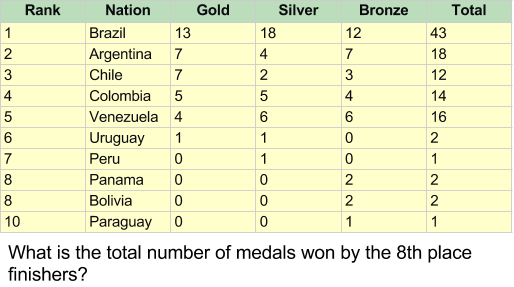
\includegraphics[width=4in]{figures/wikitables_example.png}
	\caption{Example from \WTQ{}, a dataset that does not provide
	logical form supervision}\label{fig:wikitables_example_weaksup}
\end{figure}

\paragraph{Spuriousness} The most serious challenge in building semantic parsers
with supervision only from denotations is that the search for logical forms
results in a large set of those that execute to the correct denotation, but only
coincidentally so. These are commonly referred to as spurious logical forms.

The issue is illustrated by the example from \WTQ{} shown in
Figure~\ref{fig:wikitables_example_weaksup}.
If we searched for logical forms that execute to
the correct answer (i.e., $4$), we will end up with several logical forms like
the following:

\begin{itemize}
	\item \texttt{(sum ((reverse total) (rank 8)))}
	\item \texttt{(sum ((reverse bronze) (rank 8)))}
	\item \texttt{((reverse bronze) (nation colombia))}
	\item \texttt{(count (gold 0))}
\end{itemize}

The logical form language here (and in Chapter~\ref{chapter:wikitables}) is the
$\lambda$-DCS based language introduced by~\cite{pasupat2015compositional} for
\WTQ{}. The column names are (directed) relations from cells to rows. So
\texttt{(gold 0)} refers to all the rows where the \emph{Gold} column contains
$0$. Given this, it can be see that the first logical form above is the true
translation of the question in Figure~\ref{fig:wikitables_example_weaksup},
whereas the second one returns the total number of \emph{Bronze} medals won by
\emph{Nations} ranked \emph{8}, the third one returns the number of \emph{Bronze}
medals won by \emph{Colombia}, and the last one returns the number of
\emph{Nations} that won $0$ \emph{Gold} medals, all of which return the correct
answer $4$. In fact, an exhaustive search could easily return several hundreds
of such logical forms, most of which will not be translations of original
question. Depending on the amount of supervision provided by the denotations,
this issue could be even more serious. For example, in the NLVR
dataset~\citep{suhr2017corpus} (one of the datasets we evaluate on in
Chapter~\ref{chapter:nlvr}), the denotations are binary (True or False), and
in that case, any random logical form will have a $50\%$ chance of executing to
the correct answer.

Training a semantic parser on such data will cause the model to quickly overfit to
training examples, and the algorithm used should be designed in such a way that
the model is biased away from spurious logical forms. We now describe prior
techniques used for training semantic parsers with
weak supervision, and comment on how the issue of spuriousness can be handled in
each of them.

\subsection{Maximum marginal likelihood training}\label{sec:mml}
Most work on training semantic parsers from denotations maximizes the
likelihood of the denotation given the utterance:
\begin{equation}
	\max_\theta \prod_{i=1}^N p(d_i|x_i; \theta)
\end{equation}

\noindent The semantic parsing model itself defines a distribution over
\emph{logical forms}, however, not \emph{denotations}, so this maximization
must be recast as a \emph{marginalization} over logical forms that evaluate to
the correct denotation:
\begin{equation}
	\max_\theta \prod_{i=1}^N
	\sum_{y_i \in Y_i | \llbracket y_i \rrbracket^{w_i} = d_i} p(y_i | x_i; \theta)
	\label{eq:mml_objective}
\end{equation}

\noindent This objective function is called \emph{maximum marginal likelihood}
(MML).  $Y_i$ here is the set of all valid logical forms in the world
corresponding to the $i^\text{th}$ data instance. The summation over $Y_i$ is in
general intractable to perform during training because the set $Y_i$ is too
large to enumerate, so it is only approximated.

There are two ways that this approximation has been done in prior work: (1)
using a beam search to get the best scoring parses according to the model,
hoping that at least some of those parses will yield correct denotations, and
using those parses to approximate the inner summation; or (2) performing some
kind of (typically bounded-length) heuristic search up front to find a set of
logical forms that evaluate to the correct denotation, and using those logical
forms to approximate the inner summation.  We will call the first method
\emph{dynamic MML}, because the logical forms used for the summation change
according to the current model parameters, and the second method \emph{static
MML}, as the set of logical forms used for training is fixed.  Almost all prior
work uses dynamic MML (e.g.,
\citet{liang2011learning,berant2013semantic,goldman2017weakly}).

The main benefit of dynamic MML is that it adapts its training signal over
time.  As the model learns, it can increasingly focus its probability mass on a
small set of very likely logical forms.  The main benefit of static MML is that
there is no need to search during training, so there is a consistent training
signal even at the start of training, and it can be made much more efficient
than dynamic MML\@.

Both static and dynamic MML have drawbacks, however.  Dynamic MML uses the
model to perform search, and it may not find any logical forms that evaluate to
the correct denotation, or it may only find spurious logical forms.  This
problem is exacerbated when the beam size is small, or when the model is in the
early stages of training.  Without strong lexical cues to guide the model, it
can be very difficult for the model to learn anything at all, as it blindly
searches a very large space of logical forms without any training signal until
its random search happens upon a correct logical form.  Traditionally, these
lexical cues were provided by the parser's lexicon, though with the advent of
neural semantic parsers that remove the lexicon, new techniques for providing
lexical hints need to be developed~\citep{goldman2017weakly}.

Static MML, on the other hand, relies heavily on an initial heuristic search to
find a good set of likely logical forms that evaluate to the correct
denotation.  The particulars of this heuristic search can have a large impact
on performance; a smaller candidate set will yield a better training signal,
but only if the candidate set contains the logical form that matches the
semantics of the utterance.  In the limit of a single logical form, this
becomes a fully-supervised learning problem.  However, as the size of the
candidate set decreases, the likelihood of the set actually containing the
\emph{correct} logical form also decreases.  In finding a set of candidate
logical forms, we thus need to strike a balance, keeping the set large enough
that it is likely to contain the correct logical form, but small enough to be
computationally tractable and to provide a strong training signal.
In Chapter~\ref{chapter:wikitables}, we use static MML, and leverage the dynamic
programming technique of \citet{pasupat2016inferring} to get a candidate set of logical
forms.

\subsection{Reinforcement learning methods}
When training models with discrete latent variables, a popular choice is to use
Reinforcement Learning (RL) techniques. There is a fair amount of prior work that
used RL algorithms, particularly policy gradient methods for training weakly
supervised semantic parsers. Examples
include~\cite{Andreas2016LearningTC,Liang2016NeuralSM,guu2017bridging,liang2018memory}.

These methods optimize the following objective:
\begin{equation}
	\max_{\theta} \sum_{i=1}^N \sum_{y_i \sim p(y_i|x_i;\theta)} p(y_i|x_i;\theta) \mathcal{R}(y_i)
	\label{eq:rl_objective}
\end{equation}

The problem of spuriousness can be tackled by defining a reward
function that uses some lexical or compositional cues to penalize spurious
logical forms, or designing a policy that is explicitly biased away from them.
For example,~\cite{liang2018memory} use a memory-augmented policy to explicitly store high
reward programs in a memory buffer, to bias the policy towards those.

Let us now compare objective function above with the MML objective in
Equation~\ref{eq:mml_objective}. If we define a reward function:
\begin{equation}
	\mathcal{R}_{MML}(y_i) = 
	\begin{cases}
		1, & \text{if } \llbracket y_i \rrbracket^{w_i} = d_i\\
		0, & \text{otherwise}
	\end{cases}
	\label{eq:mml_reward}
\end{equation}
we can rewrite the MML objective in Equation~\ref{eq:mml_objective} as:
\begin{equation}	
	\max_{\theta} \prod_{i=1}^N \sum_{y_i \in Y_i} p(y_i|x_i;\theta)
	\mathcal{R}_{MML}(y_i)
	\label{eq:mml_objective2}
\end{equation}
When rewritten like this, the MML objective in Equation~\ref{eq:mml_objective2} is a lot more
similar to the RL objective in Equation~\ref{eq:rl_objective}. There are two
differences that remain: First, in MML, we are maximizing a product of summations,
whereas in the RL objective, it is a sum of summations. Second, while we use
beam search or a bounded offline search to approximate the inner summation in
MML, we use sampling in RL methods.

\subsection{Structured learning algorithms}\label{sec:erm}
Since semantic parsing is a structured prediction problem, algorithms used for
other structured prediction problems may be applicable. 
There exists some prior work~\citep{IyyerSQA2016,guu2017bridging} in using 
structured learning algorithms for semantic parsing. In
Chapter~\ref{chapter:nlvr}, we consider the use of
\emph{Expected Risk Minimization} (ERM)~\citep{smith2006minimum}, which we
briefly describe here.  ERM trains a model to minimize the
expected value of an arbitrary cost function $\mathcal{C}$ as follows:
\begin{equation}
\min_{\theta} \sum_{i=1}^{N} \mathbb{E}_{p(y_i|x_i;
\theta)}\mathcal{C}(y_i) \label{eq:erm_objective}
\end{equation}

\noindent When applied to semantic parsing, estimating $p(y_i|x_i; \theta)$
could be intractable, again for the same reasons as it is for MML\@. So we use
beam search here, and approximate $p$ as $\tilde{p}$ by \emph{re-normalizing}
the probabilities assigned to all logical forms on the beam.

The fact that we can define $\mathcal{C}$ as an arbitrary cost function makes
this objective a good choice for weakly supervised semantic parsing. This lets
us incorporate additional knowledge to guide the training process,
thus effectively dealing with the issue of spuriousness. In
Chapter~\ref{chapter:nlvr}, we define the cost function as a linear combination
of a coverage measure and denotation accuracy. The coverage measure scores how
much any given logical form, $y_i$ overlaps with the functions triggered by the
utterance $x_i$. We show that this additional loss function provides a 
stronger training signal than a denotation based loss alone.

It may be noted that the ERM objective is also very similar to the RL objective
shown in Equation~\ref{eq:rl_objective}. If we expand the expectation, and 
define a reward function as follows
\begin{equation}
	\mathcal{R}_{ERM}(y_i) = -\mathcal{C}(y_i)
\end{equation}

\noindent the ERM objective becomes
\begin{equation}
	\max_{\theta} \sum_{i=1}^{N} \sum_{y_i \in Y} p(y_i|x_i;\theta)
	\mathcal{R}_{ERM}(y_i) \label{eq:erm_objective2}	
\end{equation}

\noindent So like MML, we use beam search to approximate the inner summation,
and like the policy gradient methods in RL, we use an arbitrary reward function.

\subsection{Bridging objectives}
Given the similarities among the objectives discussed so far, prior work has
explored bridging objectives to exploit the benefits of each
of them, and adapting them to specific problems.

\citet{guu2017bridging} note the
similarity between MML and RL objectives, and define a new objective that
addresses shortcomings of both MML and RL in dealing with spurious logical forms
when applied to weakly supervised semantic parsing. First, beam search in MML
has high bias when it comes to exploring paths that
lead to the correct answer, and they address this issue by injecting random
noise into exploration, like it is common in policy gradient methods. Second,
the gradient weights in RL are proportional to their current probability,
causing spurious paths to keep getting higher probability. They propose
meritocratic gradient updates to ensure all programs that obtain rewards get
upweighted equally, inspired by the fact that MML normalizes its
``rewards'' for each example. \citet{IyyerSQA2016} bridge RL techniques with
structured learning methods and
propose a reward-guided search technique for weakly supervised semantic parsing.

In Chapter~\ref{chapter:nlvr}, we describe a technique for bridging MML and
ERM, to iteratively increase the complexity of logical forms that the parser can
search for during training.
